\documentclass{article}
\usepackage[utf8]{inputenc}
\usepackage{tikz} 
\usepackage{amsfonts}
\setlength{\parindent}{15pt} % Default is 15pt.

\title{Graph Theory Reference}

\begin{document}

\maketitle
\section{Introduction}
$\mathbb{N}$ is the set of natural numbers.
The set $\mathbb{Z}/n\mathbb{Z}$ of integers
module $N$ is denoted by $\mathbb{Z}_n$.
For example, $\mathbb{Z}_2$ is
$\{\bar{0}, \bar{1}\}$. Base 2 logarithm is
written as 'log'. The expressions $x := y$ and
$y =: x$ mean that $x$ is being defined as $y$.
A partition is a set
$B = \{A_1, A_2, ..., A_k\}$ such that all sets
of $B$ are disjoint with each other. $[A]^{k}$
is the set of subsets of size $k$ in $A$.
\section{Graphs}

A graph is a pair $G = (V, E)$ of sets such
that $E \subset [V]^2$. Always assume
$V \cap E = \emptyset$. The elements of $V$ are
vertices (or nodes, or points) of the graph $G$,
while the elements of $V$ are the edges
(or lines) of graph $G$.

\begin{center}
    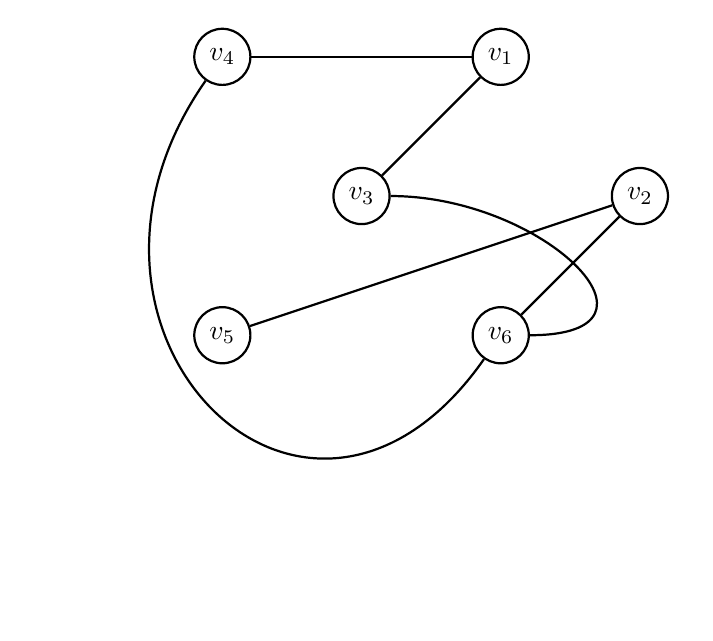
\begin{tikzpicture}[node distance={25mm},thick, main/.style = {draw, circle}]
        \node[main] (1) {$v_1$};
        \node[main] (2) [below right of=1]{$v_2$};
        \node[main] (3) [below left of=1]{$v_3$};
        \node[main] (4) [above left of=3]{$v_4$};
        \node[main] (5) [below left of=3]{$v_5$};
        \node[main] (6) [below left of=2]{$v_6$};
        \draw (2) -- (5);
        \draw (4) -- (1);
        \draw (4) to [out=235, in=235, looseness=2] (6);
        \draw (3) to (1);
        \draw (2) to (6);
        \draw (6) to [out=0, in=0, looseness=2] (3);
    \end{tikzpicture}\\
    \emph{The graph on $V = \{v_1, \ldots, v_6\}$
        with edge set
        $E = \{\{v_1, v_4\}, \{v_1, v_3\}
            , \ldots, \{v_4, v_6\}\}$}
\end{center}

A graph with vertex set $V$ is said to be a graph
on $V$. The vertex of a graph G is referred to as
$V(G)$, its edge set as $E(G)$. Sometimes, a graph
might not be distinguished from its edge and vertex
set. For example, a vertex $v \in G$ instead of
$v \in V(G)$, and an edge $e \in G$ instead of
$e \in E(G)$.

The number of vertices of a graph G is its order,
written as $|G| = |V(G)|$; its number of edges
is denoted by $||G|| = |E(G)|$. According to the graph's
order, they are finite, infinite, countable and so on.

The empty graph $(\emptyset, \emptyset)$ is
denoted simply as $\emptyset$. A graph with order
0 or 1 is called trivial. Trivial graphs are useful
e.g. to start an induction; they are also silly
counterexamples. The text generally disregards
the trivial graphs.

A vertex $v$ is incident with an edge $e$ if $v \in e$;
then $e$ is an edge at $v$. An edge $\{x, y\}$
is usually written as $xy$ or $yx$. If $x \in X$
and $y \in Y$, then $xy$ is an $X-Y$ edge. The
set of all $X-Y$ edges in a set $E$ is denoted by
$E(X, Y)$; instead of $E({x}, Y)$ and $E(X, {y})$
we simply write $E(x, Y)$ and $E(X, y)$. The
set of all edges in $E$ at a vertex $v$ is denoted
by $E(v)$.

Two vertices $x, y$ of $G$ are adjacent, or neighbors,
if ${x, y} \in E(G)$. Two edges $e \neq f$ are
adjacent if they have an end in common
($e \cap f \neq \emptyset$). If all the vertices
of G are pairwise adjacent, then $G$ is complete.
A complete graph on $n$ vertices is a $K^n$;
a $K^3$ is called a triangle.

Pairwise non-adjacent vertices are independent.
A set of vertices or edges is independent if
no two elements of its elements are adjacent.
Independent sets of vertices are called stable.

Let $G = (V, E)$ and $G' = (V', E')$ be two graphs.

\end{document}